\chapter{Weyl semimetals}

\section{Physical aspects}


\section{Topological description}

%TODO introductory paragraph

\subsection{3D Chern insulators}

%TODO incorporate feedback

To get a good intuition for the topological description of Weyl semimetals, it will be useful to consider a fully insulating material with similar properties first. That is, suppose we have a three-dimensional material that is not subject to any additional symmetries. Such a material is called a 3D Chern insulator, in analogy to the 2D Chern insulator studied in Section \ref{sec:Chern}.%TODO
This is not a semimetallic phase in the sense that there are no band crossings in the bulk; still, in some sense it can be considered a limiting case of a Weyl semimetal, where the number of Weyl points is zero.

From the Atland--Zirnbauer classification in Table \red{[reference]},%TODO
one might expect a 3D Chern insulator to be topologically trivial. However, as seen before in equation \red{[reference] (and perhaps also in 3D BHZ/Kane--Mele if I discuss this in ch. 2)},%TODO
the full topological classification of materials depends not only on the top-dimensional topology, but also on that borrowed from lower-dimensional subspaces. In the case of a 3D Chern insulator, this topology arises on two-dimensional slices of the Brillouin zone; an example of such a slice is highlighted in Figure \ref{fig:3D_Chern_insulator}.
\begin{figure}[htb!]
	\centering
	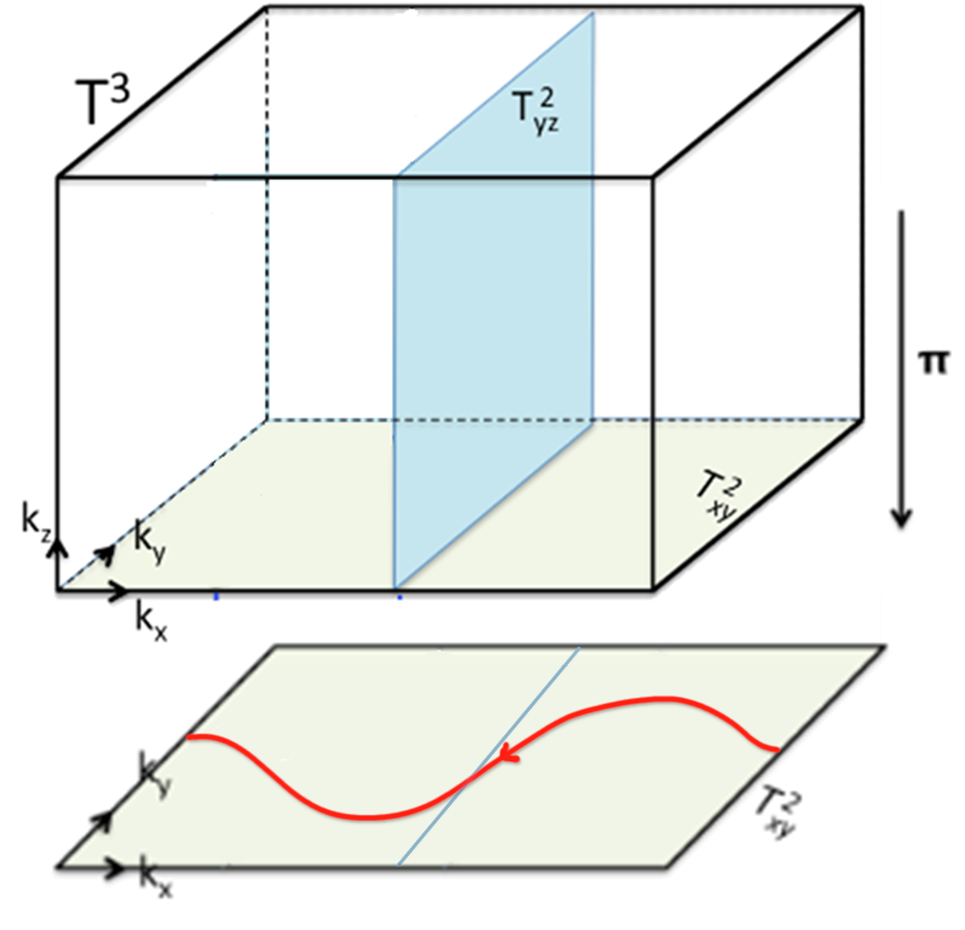
\includegraphics[width=.5\linewidth]{Images/3D_Chern_insulator}
	\caption{
		\red{[Temporary figure]} %TODO fix
		Three-dimensional Brillouin torus $\T^3$ of a Chern insulator, with a two-dimensional slice $\T_{yz}^2$ indicated in blue. A projection onto a surface Brillouin zone in the $xy$-direction is also shown, with an example Fermi loop of gapless states in red. In this example, the slice $\T_{yz}^2$ has a Chern number of $C_{x} = 1$, and so its projection onto the surface is a 1D loop that features one band crossing.
		Figure adapted from \cite{Mathai_math-review}.}
	\label{fig:3D_Chern_insulator}
\end{figure}

There are three topologically distinct ways to slice up the three-torus, all perpendicular to one of the three coordinate directions.\footnote{
	Other 2D slices exist, such as those going diagonally across, but these can all be considered linear combinations of the three ``orthogonal'' slices. To be precise, the different classes of 2D subspaces of $\T^3$ form the second homology group $H_2(\T^3)\cong\Z^3$, and this group is \emph{generated} by the orthogonal slices.}
These slices have the topology of a two-torus $\T^2$, and a Chern number can be obtained by integrating the Berry curvature $\Fc$ of the system over them: for example, perpendicular to the $x$ direction we obtain $C_{x} = \int_{\T_{yz}^2}\mathcal{F}$.\footnote{
	Note that it does not matter where along the Brillouin zone this $yz$-slice is taken: the Chern number is an integer, while the system is continuous. This means the $x$ coordinate can be changed continuously without changing the resulting Chern number.}
This results in a classification by three distinct Chern numbers $C_x$, $C_y$ and $C_z$, and in the literature (e.g. \cites{Vanderbilt_2018}{Liu_photonic-Chern-vector}) these are commonly arranged in a so-called \emph{Chern vector}
\[
	\vb{C} = \begin{pmatrix}
		C_x \\ C_y \\ C_z
	\end{pmatrix} \in \Z^3.
\]

Importantly, these three Chern numbers are all induced by a single two-form $\Fc$. In this sense, there is an exact correspondence between topologically distinct Berry curvatures $\Fc$ and Chern vectors $\vb{C}\in\Z^3$. This is precisely what motivates the use of cohomology for classification: just like in the 2D Chern insulator, the two-form $\Fc$ can be considered to represent a class in the second cohomology group:
\begin{equation}
	[\Fc]\in H^2(\T^3)\cong\Z^3. \label{eq:2nd-cohom-z3}
\end{equation}
As a result, this group precisely classifies the distinct topological phases of the system.\footnote{
	More fundamentally, a complex vector bundle called the \emph{valence bundle} can be associated to a gapped Hamiltonian, and the second cohomology group classifies the different complex vector bundles over a manifold.}

\subsubsection{Boundary states}

Before moving on to a system with Weyl points, it will be instructive to study the gapless modes that arise on the surface of a 3D Chern insulator with non-zero Chern vector. Figure \ref{fig:3D_Chern_insulator} illustrates the case where $\vb{C} = (1,0,0)\tran$. In this case, $\T_{yz}^2$ is the only orthogonal slice with a non-zero Chern number, and as such the material lattice can be thought of as a stack of 2D Chern insulators spanning the $y$ and $z$ directions, stacked together in the $x$ direction. $\T_{yz}^2$ can effectively be considered the Brillouin zone of such a 2D Chern insulator.

Recall from our discussion in Section \ref{sec:Chern} that a 2D Chern insulator with a Chern number of 1 has a single chiral edge mode, which manifests as a gapless state on the one-dimensional surface Brillouin zone. %TODO Extra canceling edge modes may appear <=> folding of the Fermi loop
This logic can be translated to the the three-dimensional case, where such slices are stacked in the $x$ direction. Suppose there is a projection $\pi$ along the $z$ direction, onto a two-dimensional surface Brillouin zone $\ext{\T}_{xy}^2$. Then the two-dimensional slices $\T_{yz}^2$ project down to a one-dimensional loop $\pi(\T_{yz}^2)\cong S^1$ containing a single point-like gapless state. As the $\T_{yz}^2$ slice is moved around in the $x$ direction, this band crossing point moves continuously along the $y$ direction, by continuity of the Hamiltonian. It follows that the full two-dimensional surface Brillouin zone must contain a loop of gapless states going across the $x$ direction, as depicted in the figure. This loop is called a Fermi loop, in analogy with the Fermi arcs in a Weyl semimetal, and the existence of such loops is experimentally well documented \red{[references]}. %TODO refs
Moreover, the chirality of the edge modes can be used to assign a consistent orientation to this loop. %TODO note about linked loops, extra topology etc.

Fermi loops admit a natural topological description in terms of homology. Being oriented loops, they precisely represent a class in the first homology group $H_1(\ext{\T}^2)$ of the surface Brillouin zone. Furthermore, it is possible to define an oriented \emph{Dirac loop} %TODO terminology
$\ell$ in the bulk Brillouin zone in such a way that its projection $\pi(\ell)$ onto the surface in any direction is exactly the Fermi loop. This loop $\ell$ represents a first homology class in the bulk Brillouin zone,
\[
	[\ell]\in H_1(\T^3)\cong\Z^3.
\]

It is not a coincidence that this first homology group is isomorphic to the second cohomology group $H^2(\T^3)$ from Equation (\ref{eq:2nd-cohom-z3}). This equivalence is a result of \emph{Poincaré duality}, which is the statement that for any closed oriented $d$-dimensional manifold $M$, the isomorphism
\[
	H_n(M) \cong H^{d-n}(M)
\]
holds for any integer $n$. In the present case, this duality can be stated intuitively in terms of Chern numbers, which count the number of signed intersections of the Dirac loop with the different two-dimensional slices of the Brillouin zone. This duality can be summarised schematically as follows:
\[
	H^2(\T^3) \ni [\Fc] \overset{\rm integration}{\iff} \vb{C} \overset{\rm intersections}{\iff} [\ell] \in H_1(\T^3).
\]
This Poincaré duality ensures that the classifications in terms of first homology and second cohomology are completely equivalent in this case. Importantly, however, Poincaré duality depends on orientability, and it will not hold when we consider non-orientable Brillouin zones in the next chapter. As such, the question of which group provides the right classification of such a system will be key. For the moment, we turn our attention to the topology of Weyl points in the simpler orientable setting.


\subsection{Introducing Weyl points}

Consider a Weyl semimetal with a set of $k$ Weyl points
\[
	W \equiv \set{w_1,w_2,\ldots,w_k}\subset \T^3.
\]
Then the charge of a Weyl point $w_i$ is given by the Chern number
\begin{equation}
	C_w = \int_{S_w^2}\!\Fc,
\end{equation}
where $S_w^2$ is a sufficiently small 2-sphere centred at $w$---in particular, it must be small enough to contain no other Weyl points in its interior. The Nielsen--Ninomiya charge cancellation theorem is the statement that all these charges must add to zero:
\begin{equation}
	\sum_{i=1}^{k}C_{w_i} = 0.
\end{equation}
This cancellation can be demonstrated using Stokes' theorem. The argument goes as follows: imagine the small open 3-ball bounded by $S_w^2$ is removed from $\T^3$ around each Weyl point $w$. The resulting 3-manifold $X$ looks like a 3-torus with small holes, and its boundary is given by the collection of 2-spheres around the Weyl points:
\[
	\partial X = -\bigcup_{i=1}^k S_{w_i}^2,
\]
where the minus sign induces the correct orientation. Then Stokes' theorem gives
\[
	0 = \int_{\partial X} \dd{\Fc} = -\sum_{i=1}^{k}\int_{S_{w_i}^2}\!\!\Fc = -\sum_{i=1}^{k}C_{w_i}.
\]

A similar argument can also be applied to study what happens to Chern numbers on two-dimensional slices of the Brillouin zone when Weyl points are introduced. This argument is illustrated in Figure \ref{fig:Weyl-point-Stokes}.
\begin{figure}[htb!]
	\centering
	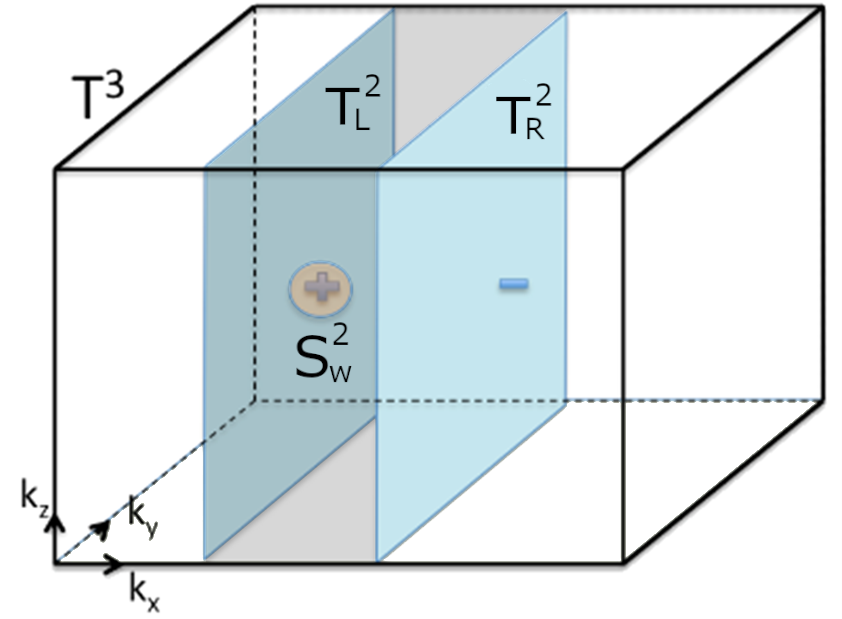
\includegraphics[width=.5\linewidth]{Images/Weyl-point-Stokes}
	\caption{
		Brillouin torus $\T^3$ of a Weyl semimetal with two oppositely charged Weyl points labelled $+$ and $-$. Three two-dimensional subspaces are indicated in blue: a $yz$-like 2-torus on either side of the $+$ point, and a small 2-sphere surrounding it. Given the proper orientation, the blue spaces form the boundary of a three-dimensional manifold $Y$, shaded in grey here.
		Figure from \cite{Mathai_math-review}. \red{[not yet licensed; may need better labelling]}%TODO
	}
	\label{fig:Weyl-point-Stokes}
\end{figure}
Here two slices $\T_L^2$ and $\T_R^2$ are placed on either side of a Weyl point $w$ with charge $C_w = q$, along with a small sphere $S_w^2$ surrounding it. These spaces then bound a three-dimensional manifold $Y$ as indicated in the figure, given the following orientations:
\[
	\partial Y = \T_R^2 - \T_L^2 - S_w^2.
\]
The same Stokes' theorem argument can then be used to relate the Chern numbers $C_L$ and $C_R$ on the respective slices, yielding
\[
	C_R = C_L + C_w = C_L + q.
\]
That is, the Chern number of a two-dimensional slice increases by $q$ every time it passes over a Weyl point with charge $q$. As a sanity check, it should be noted that this process respects the periodicity of the Brillouin torus: indeed, when the slice is passed over the entire torus, charge cancellation ensures that the added Chern number is zero in total.

All in all, the presence of Weyl points allows for a finer collection of Chern numbers to appear in the Brillouin zone, beyond the $\Z^3$ Chern vector of the insulating case. This behaviour can be captured using cohomology. The key idea is that the Berry curvature can only be integrated over subspaces where the gap never closes, so that the set of Weyl points $W$ needs to be excluded. To be precise, we are interested in classifying possible Chern numbers on $\T^3\setminus W$, the Brillouin zone minus $W$; these correspond precisely to all possible gapless phases on $\T^3\setminus W$. This means the Berry curvature now lives in the second cohomology group of this space:
\begin{equation}
	[\Fc]\in H^2(\T^3\setminus W) \cong \Z^3\oplus\Z^{k-1},
\end{equation}
where $k$ again is the number of Weyl points. It follows that there are $k-1$ extra factors of $\Z$ involved in the classification of a Weyl semimetal compared to that of a 3D Chern insulator. One might expect this to be $k$ factors, but the reduction by one is a natural result of Nielsen--Ninomiya: for example, if $k=1$ then charge cancellation implies that the single Weyl point must have a charge of 0, and so it is not topologically protected.


\subsubsection{Fermi arcs}

The varying Chern numbers over Weyl points help explain how Fermi arcs arise on the surface. As discussed in the case of a 3D Chern insulator, Fermi loops on the surface arise whenever there is a non-zero Chern number in some direction. Similarly, Fermi arcs begin and terminate whenever the presence of a Weyl point causes a change in the Chern number; this is illustrated in Figure \ref{fig:Fermi-arc-Chern}.
\begin{figure}[htb!]
	\centering
	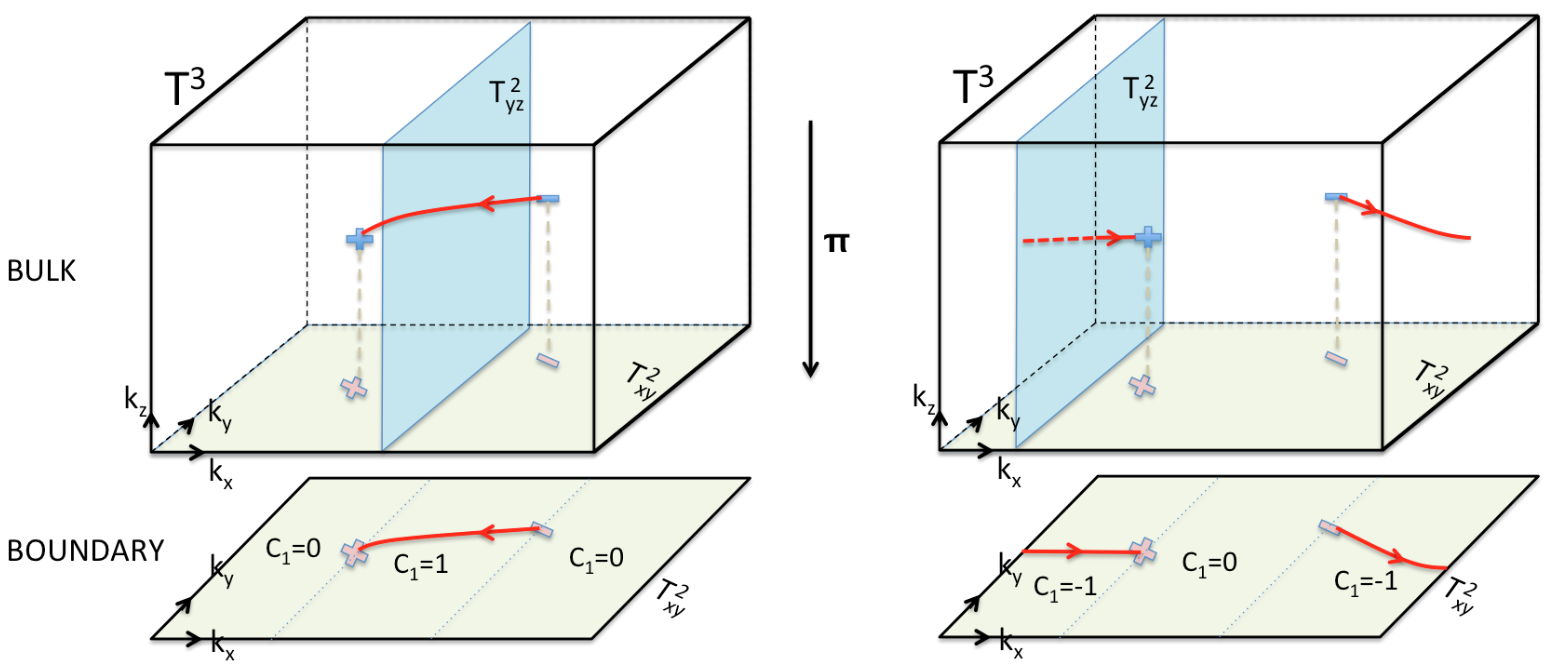
\includegraphics[width=\linewidth]{Images/Fermi-arc-Chern}
	\caption{
		Two semimetal Brillouin zones are shown with the same configuration of Weyl points, but featuring topologically distinct Fermi arcs (shown in red on the boundary). The distinction is due to different bulk Chern numbers: Fermi arcs appear in regions where the bulk Chern number is non-zero. These Fermi arcs can be considered to be the projection of a Dirac string (shown in red in the bulk).
		Figure from \cite{Mathai_math-review}.}
	\label{fig:Fermi-arc-Chern}
\end{figure}

\subsection{The Mayer--Vietoris sequence}